% -*- mode: LaTeX; coding: utf-8; -*-

\chapter{Dynaamiset Web-teknologiat}

Internet on aina ollut vihamielinen paikka, jossa sivustolla vierailevan motiiveja sivustoa ja palvelua kohtaan on mahdotonta ennustaa. Tästä syystä 
useimmat kehittäjät ja ylläpitäjät ovat noudattaneet periaatetta, että kehenkään ei voi täysin luottaa. Sivustojen ja palveluiden kehittyessä entistä monimutkaisemmiksi, on tämän 
luottamattomuusperiaatteen noudattaminen noussut entistä tärkeämmäksi.

Webin teknisen monimutkaistumisen taustalla on dynaamisuuden lisääntyminen. Paljon sellaisia tehtäviä, jotka aiemmin olivat palvelimen vastuulla, on siirretty käyttäjän selaimessa 
suoritettavaksi. Lisäksi Web-sivujen sisältö ei ole enää staattista, vaan uutta sisältöä voidaan ladata sivulle käyttäen useitakin eri teknologioita. Vaikka kasvava määrä tietoturvahyökkäyksistä 
tapahtuu dynaamisten Web-teknologioiden avulla, ei se tarkoita sitä, että ne olisivat tietoturvan kannalta normaalia heikompia tai, että ne sisältäisivät helposti hyödynnettäviä 
haavoittuvaisuuksia. Dynaamisuus vain mahdollistaa aikaisempaa joustavamman alustan toteuttaa interaktiivisia ja normaalien työpöytäsovelluksien 
kaltaisia palveluita, joita käyttäjät voivat ajaa suoraan Web-selaimesta. Varsinainen ongelma piilee siinä, että dynaamiset Web-palvelut ovat aikaisempaa monimutkaisempia toteuttaa. Niissä 
hyödynnetään useita eri teknologioita ja rajapintoja, jonka johdosta mahdollisuus tehdä virheitä kasvaa verrattaessa vanhoihin ratkaisuihin. Käytetyt teknologiat eivät siis ole syynä 
heikentyneeseen tietoturvatasoon, vaan syynä on kehittäjien huolimattomuus tai tietämättömyys niistä mahdollisuuksista, joita huonosti suunnitellut ja toteutetut palvelut avaavat hyökkääjille.

\section {AJAX}

Jos jokin dynaamisista Web-teknologioista halutaan nostaa kehitystä eniten eteenpäin vieväksi voimaksi, niin vahvin ehdokas tähän on Asynchronous JavaScript and XML (lyh. AJAX). Se
itsessään ei ole mikään yksi tietty teknologia, vaan se on usean eri teknologian yhdistelmä, joita käyttämällä Web-sivut pystytään muuttamaan nopeasti reagoiviksi ja niiden 
käyttökokemus saadaan muistuttamaan perinteisiä työpöytäsovelluksia \cite{AJAX}. AJAX koostuu seuraavista teknologioista:

\begin{itemize}
\item HTML ja CSS rakentavat Web-selaimella näytettävän sivun.
\item DOM mahdollistaa ajonaikaisen sisällön tuottamisen.
\item XML ja Extensible Stylesheet Language Transformation (lyh. XSLT)
  mahdollistavat eri komponenttien välisen tiedonsiirron.
\item JavaScript helpottaa eri komponenttien integroimista sekä näiden
  ohjelmoimista.
\item XMLHttpRequest (lyh. XHR) -olio helpottaa kommunikointia
  palvelinten kanssa \cite{WEB2b}.
\end{itemize}

Suurin AJAXin tuoma muutos perinteisiin Web-sivuihin on mahdollisuus päivittää sivun sisältöä asynkronisesti ilman käyttäjän vuorovaikutusta. Yksinkertaistettuna tämä tarkoittaa sitä,
että sivun sisällöstä pystytään päivittämään ainoastaan halutut osat käyttäen XHR-kyselyitä. Aikaisemmin tällainen ei ole ollut mahdollista, sillä vanhat Web-sivut toimivat
pelkästään synkronisesti, jolloin erillisiä kutsuja ei voitu tehdä. Tällöin koko sivu täytyi päivittää kerralla. Tämä on ollut käytettävyyden kannalta huono asia,
sillä sivu ei ole synkronisen latauksen ja käsittelyn aikana käytettävissä. XHR sisältää kaikki perinteiset HTTP-metodit mukaan lukien GET, POST, HEAD ja DELETE, joten sen avulla 
pystytään suorittamaan kaikki yleisimmät käyttäjän toiminnot \cite{WEB2}. Kuvassa \ref{synkroninen} on esitetty tilanne, jossa sama palvelu on toteutettu käyttäen synkronisia ja 
asynkronisia kutsuja. Kuvasta voi havaita, että dynaamisuus mahdollistaa useamman samanaikaisen kutsun tekemisen, jolloin myös palvelun viiveet voidaan pitää lyhyinä.

\begin{figure}[htp]
\centering
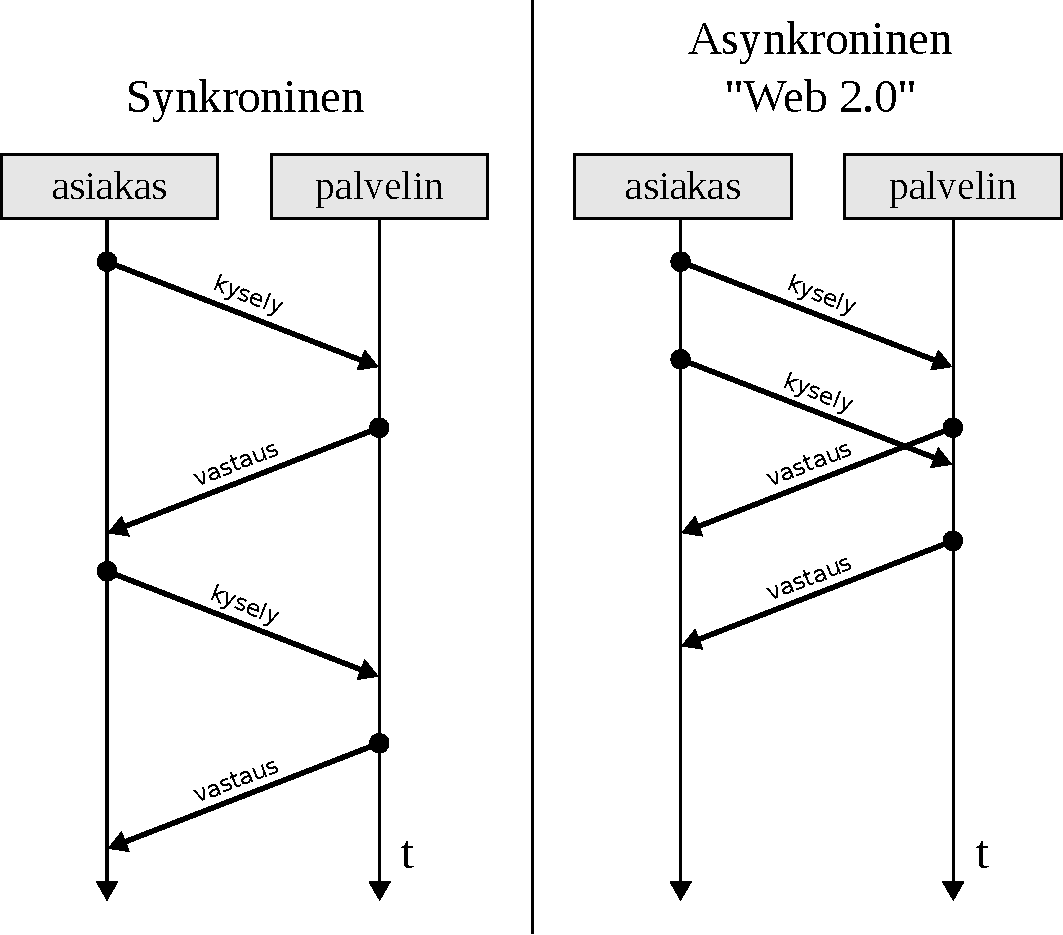
\includegraphics[width=11.5cm]{pics/synkroninen.pdf}
\caption{Synkroninen ja asynkroninen kommunikointi.}
\label{synkroninen}
\end{figure}

AJAXiin kohdistuvat hyökkäykset eivät eroa suuresti vanhoista murtautumismenetelmistä. Hyökkääjät pyrkivät edelleen hyödyntämään syötteen puutteellista suodattamista, muokkaamaan 
ulos tulevaa dataa, murtamaan salauksia ja hankkimaan istuntokohtaisia tietoja esimerkiksi evästeitä varastamalla. Hyökkääjien näkökulmasta AJAXin tekee erityisen kiinnostavaksi se,
että aiempaa suurempi osa Web-palvelun käyttämästä laskennasta suoritetaan käyttäjän selaimessa. Käyttäjän selaimeen, eli niin sanottuun asiakaspuoleen, ei voida kuitenkaan koskaan luottaa.
JavaScriptien huolimaton käyttö avaakin hyökkääjille lukuisia tapoja murtautua palveluihin. Kyseessä on sinänsä pitkään tunnettu ongelma, mutta kehittäjien kiinnostuksen siirtyessä 
AJAXiin ovat myös hyökkääjät alkaneet kiinnittämään asiaan enemmän huomiota \cite{AJAX}. Monet käytetyistä AJAX-ympäristöistä sisältävät myös eriasteisia tietoturvariskejä, joita 
hyökkääjät voivat hyödyntää \cite{JSH}.

\subsection{JavaScript}

JavaScript on Netscapen suunnittelema skriptikieli, joka tunnettiin aluksi nimellä LiveScript. Sun Microsystemsin kehittämän Java-ohjelmointikielen yleistyessä Net\-scape päätti muuttaa
sen nimen JavaScriptiksi toivoen sen käytön yleistyvän Javan menestyksen myötä. JavaScriptillä kirjoitetut skriptit sijoitetaan HTML:n \texttt{<script>}-elementin sisään, josta voi 
olla myös viite erilliseen lähdekooditiedostoon. JavaScript vaatii tuen selaimelta, jollainen löytyy miltei jokaisesta Web-\-selaimesta mukaan lukien yleisimmät mobiililaitteet.

JavaScript on tehokas työkalu, joka mahdollistaa monen muun toiminnon ohella muun muassa dynaamisten Web-sivujen tekemisen, viestien kirjoittamisen selaimen tilariville, uusien ikkunoiden
avaamisen ja interaktiivisten lomakkeiden luomisen. Skriptien toiminta rajoittuu kuitenkin Web-selaimen toimintoihin, eikä sitä käyttäen voida esimerkiksi kirjoittaa levylle ja levyn 
lukeminen rajoittuu pelkästään evästeisiin \cite{JavaScript}. Näistä rajoituksista huolimatta JavaScript mahdollistaa erittäin monipuolisten toimintojen toteuttamisen Web-ympäristössä.

Suurin osa Web-sivuilla olevista skripteistä toimii siten, että ne ladataan aluksi käyttäjän koneelle, jonka jälkeen ne suoritetaan selaimessa. Skriptit sijaitsevat ja ne suoritetaan 
käyttäjien koneilla, joten toimintaperiaatteen selvittäminen ei ole hyökkääjälle vaikeaa. Asiaa pystytään kuitenkin vaikeuttamaan muutamalla eri tavalla. Näistä yksinkertaisin on 
\emph{obfuskointi}, jonka yhteydessä koodista tehdään vaikeasti luettavaa. Aluksi poistetaan kommentointi ja tyhjät rivivälit, seuraava askel on koodin muuttujien ja objektien
uudelleen nimeäminen, jolloin hyökkääjän on vaikeampi päätellä näistä skriptin toimintaperiaate. Nimet voidaan myös muuttaa esimerkiksi binäärikoodiksi. Nämä keinot ovat kuitenkin 
vain hidasteita osaavalle hyökkääjälle \cite{AJAX}. Palvelu tulisikin suunnitella siten, että kaikki luottamuksellisen tiedon käsittely ja käyttäjän syötteen tarkistukset suoritettaisiin
Web-palvelimella. Tällöin käyttäjän selaimessa suoritettaisiin ainoastaan sellainen laskenta, joissa käsitellään käyttäjää itseään koskevaa dataa.

Koneelle ladatut skriptit ajetaan oletuksena hyvin rajatussa tilassa, jossa niillä on pääsy vain kyseistä sivun sisältämään dataan tai siihen hyvin läheisesti kuuluviin dokumentteihin. 
JavaScript noudattaa myös  edellisessä luvussa esitettyä \emph{saman alkuperän} periaatetta, joka estää skriptien suorittamisen muista Internet-domaineista kuin siitä, josta skripti on
ladattu. Näin vaikeutetaan hyökkäyksen tekemistä käyttäen toiselta sivulta ladattua haitallista skriptiä, jonka avulla voitaisiin esimerkiksi varastaa evästeitä ja urkkia näppäimistön
painallukset.  Aikaisemmin selaimet ovat sallineet joitain poikkeuksia tähän periaatteeseen, mutta tietoturvasyistä nämä on kuitenkin poistettu.

Liian tiukat tietoturvasäännöt eivät 
kuitenkaan toimi nykyaikaisten Web-\-palveluiden kanssa, ja tästä syystä \emph{saman alkuperän} periaatetta on mahdollista löysentää. Esimerkiksi ulkoiset linkit, jotka osoittavat toisella
sivustolla olevaan skriptiin, ohittavat \emph{saman alkuperän}, sillä vaikka itse skripti sijaitsee toisella palvelimella niin se lasketaan kuuluvan siihen sivuun, jossa viittaus
lähdekooditiedostoon on.  Näin kutsutulla skriptillä on pääsy sellaisiin evästeisiin ja tiedostoihin, joihin sillä ei välttämättä tarvitsisi olla oikeuksia. Sivustojen ja palveluiden 
käyttäessä resursseja entistä useammasta lähteestä eri palvelimilta, voi tämä aiheuttaa riskitilanteita, jos jonkin lähteen tietoturva on vaarantunut \cite{AJAX}.

\subsection{AJAXiin liittyvät tietoturvariskit}

Koska AJAXin toiminta perustuu hyvin pitkälti JavaScriptin varaan, on itsestään selvää, että hyökkääjät pyrkivät väärinkäyttämään ensisijaisesti JavaScriptin haavoittuvaisuuksia.  
Asiaa ei auta se, että suurin osa sivustoista on jollakin tavalla alttiina XSS-hyökkäyksille \cite{WEB2c} johtuen huonosti toteutetusta syötteen tarkistuksesta. Asetettuja suodatuksia 
pystytään myös kiertämään käyttäen esimerkiksi kuvalinkkejä ja monia HTML-elementtejä, joiden avulla ajettava skripti voidaan hukuttaa muun syötteen joukkoon. Tästä syystä pelkästään 
tiettyjen merkkijonojen suodattaminen ei takaa suojaa JavaScript-pohjaisilta hyökkäyksiltä. Tehokkain ja yksinkertaisin keino onkin poistaa kaikki HTML-elementteihin kuuluvat merkit, 
jolloin esimerkiksi \texttt{<}-merkistä tulee \texttt{\&lt;} ja \texttt{>}-merkistä \texttt{\&gt;}. Monet ympäristöt mahdollistavat myös suoraan HTML-elementtien poistamisen käyttäjien
jättämistä viesteistä \cite{AJAX}. Tällöin esimerkiksi foorumeilla toisten käyttäjien lähettämistä viesteistä saadaan estettyä niiden mahdollisesti sisältämän JavaScript-ohjelmakoodin
suorittaminen.

Kasvaneella JavaScriptin käytöllä on suora vaikutus myös XSS-hyökkäysten yleistymiseen. JavaScriptillä pääsee helposti evästeisiin käsiksi käyttäen \emph{document.cookie}-oliota. 
Vaikka sen käyttö on rajoitettu ainoastaan sen Internet-domainin evästeeseen, josta kutsu on tehty, voidaan tämä rajoitus ohittaa melko helposti. Hyökkääjälle riittää, että käyttäjä 
vierailee esimerkiksi sellaisessa foorumissa tai blogissa, joissa käyttäjien viesteissä sallitaan XHTML:n käyttö. Tämä mahdollistaa haitallisten skriptien lähettämisen sivustolle ja pahaa
aavistamaton käyttäjä, joka vierailee tällä sivulla, joutuu tietämättään hyökkäyksen kohteeksi.

Yksi tapa suojautua evästeiden varastamiselta on käyttää HTTP-only~-evästeitä, jolloin käyttäjien evästeitä ei pystytä lukemaan JavaScriptillä. Näiden evästeiden tukeminen on kuitenkin selainkohtaista,
joten tämä ratkaisu ei aina välttämättä ole mahdollista toteuttaa. XSS-hyökkäykset eivät myöskään rajoitu pelkästään evästeiden varastamiseen, ja yhtä helposti hyökkääjä voi esimerkiksi
luoda skriptin, joka lukee näppäimistön painallukset ja lähettää ne haluttuun osoitteeseen. HTTP-only -evästeiden käyttö ei myöskään täysin suojaa evästeitä, jos käytetään XHR-kutsuja. 
Tällöin hyökkääjän on mahdollista lukea suoraan otsaketiedoissa asetettuja arvoja. Jotkut XHR-objekteihin liittyvät haavoittuvuudet ovat myös niin syvällä XHMLHttpRequest-objekteissa, että 
kaikki nykyisin käytössä olevat toteutukset ovat niille jossakin määrin alttiina. Kaapattujen XHR-objektien tunnistaminen ei myöskään vielä ole mahdollista \cite{AJAX}. Näistä syistä johtuen 
AJAX tarjoaa nyt ja tulevaisuudessa hyökkääjille monia mahdollisuuksia murtaa asetettuja suojauksia.

Yksi yleisimmistä AJAX-ohjelmoinnissa käytetyistä tiedon esitystavoista on JavaScript Object Notation (lyh. JSON). Se on ohjelmointikielestä riippumaton ja laajasti tuettu Web-palvelimella käytetty 
työkalu. Se on rakenteeltaan hyvin kevyt ja se koostuu kahdesta eri tietotyypistä: olioista ja taulukoista \cite{JSON}. Formaatin heikkous piilee siinä, että JSON-olio itsessään on kelvollinen 
JavaScript-ohjelma, jonka sisältö on mahdollista kaapata \cite{AJAX}. Termi \emph{JavaScript Hijacking} kuvaa tällaista tilannetta, jossa hyökkääjä ohittaa \emph{saman alkuperän} periaatteen 
silloin, kun JavaScriptiä käytetään arkaluontoisen tiedon lähettämiseen. Aiheesta tehdyn tutkimuksen \cite{JSH} mukaan lähes jokainen käytetty AJAX-ympäristö on alttiina tällaisilla hyökkäyksille.
Käyttäen CSRF-hyökkäystä hyökkääjä pystyy väärinkäyttämään JSON-formaattia, ja varastamaan sekä muokkaamaan toiselle sivustolle lähetettäviä paketteja.  Tällainen hyökkäys voidaan toteuttaa 
useilla eri tavoilla mukaan lukien käyttäen \texttt{<script>}-elementtiä, ja koska pyyntö tulee selaimen luottamasta lähteestä, voidaan tällä tavoin ohittaa esimerkiksi SSL-suojaus\cite{AJAX}.

Suojautuminen tämän tyyppisiltä hyökkäyksiltä voidaan toteuttaa monella eri tapaa, ja paras tulos saadaan yhdistelemällä näitä. Koska CSRF-hyökkäyksessä hyökkääjä joutuu toimimaan osittain 
sokeasti, voidaan jokaiseen pyyntöön lisätä parametri, jota hyökkääjän on vaikea arvata. Palvelin voidaan myös asettaa tarkistamaan HTTP Referer -kenttä, jolla voidaan varmistaa, että pyyntö 
tulee sallitulta taholta, vaikkakin Referer-kentän sisältö voidaan helposti muuttaa. Toinen tapa on muokata vastaanottopäässä paketteja siten, että hyökkääjä ei pysty ajamaan lähettämissään 
pyynnöissä skriptejä 
\cite{JSH}.

\section{Flash}

AJAXin ohella Macromedian suunnittelema, ja nykyisin Adoben kehittämä Flash, on ollut yksi niistä merkittävistä tekniikoista, joita käyttämällä YouTuben ja MySpacen kaltaiset 
menestyspalvelut ovat olleet mahdollisia toteuttaa. Flashia käyttämällä kehittäjät ovat jo pitkään pystyneet luomaan interaktiivista ja rikasta Web-sisältöä
yksinkertaisista animaatioista aina monimutkaisiin peleihin ja valikoihin asti. Suurin osa Web-sivustoilla olevista mainoksista on myös toteutettu käyttäen Flashia. Näistä syistä johtuen 
Flash Player on yksi ohjelmistoalan de facto~-tekniikoista, jonka käyttöaste yritys- ja kuluttajapuolella on lähes 100 prosenttia \cite{Flash}.

Flashin käyttämä ActionScript-skriptikieli muistuttaa läheisesti JavaScriptiä ja sitä käyttäen on mahdollista luoda uusia TCP-yhteyksiä, ajaa JavaScriptiä selaimessa ja luoda 
sallittuihin domaineihin HTTP-pyyntöjä. Flashin käyttämä tietoturvamalli noudattaa paljolti \emph{saman alkuperän} periaatetta, jolla rajoitetaan eri domaineissa sijaitsevien sovellusten 
kommunikointia. Domainien välinen kommunikointi on kuitenkin sallittua, ja käytetty tietoturvapolitiikka luetaan tähän tarkoitetusta XML-tiedostosta. Tämä XML-tiedosto sijaitsee usein 
domainin juuressa ja se sisältää ne domainit, jotka saavat olla siihen yhteydessä. Osa Flashiin kohdistuvista hyökkäyksistä pyrkiikin muokkaamaan tietoturvapolitiikkatiedoston sisältöä
siten, että kohde sallisi yhteydet myös hyökkääjän käyttämästä osoitteesta. Tämä voidaan toteuttaa esimerkiksi käyttämällä vihamielistä RSS-syötettä tai luomalla tiedosto, joka sisältää
uuden XML-tiedoston. Yksi tällaisista hyökkäyksistä on Stefan Esserin luoma GIF-tiedosto, jonka kommenttiin on piilotettu uusi tietoturvapolitiikka. Hyökkääjälle riittää, että kohdekone 
vain mahdollistaa tiedoston lataamisen palvelimelle, jonka jälkeen vanha sisältö voidaan korvata GIF-tiedostoon piilotetulla \cite{WEB2}.

Perimmäinen syy sille, miksi XSS-hyökkäykset ovat yleistyneet viime vuosina on se, että käyttäjien antamaa syötettä ei usein tarkisteta riittävällä tarkkuudella. Sama pätee myös suureen 
osaan Flash-pohjaisista toteutuksista, joihin käyttäjien on mahdollista antaa syötteitä. Tämä avaa useita erilaisia Flashia hyödyntäviä XSS-hyökkäyksiä, jotka pyrkivät väärinkäyttämään 
käyttäjän selaimen ja sivuston välistä luottamussuhdetta. Aina vika ei ole Flash-toteutuksen tekijässä, sillä Flash-tiedostoja luodaan usein automaattisesti käyttämällä valmiita 
sovelluksia. Aiheesta tehdyn kattavan tutkimuksen mukaan \cite{FlashXSS} suurimmasta osasta näin luoduista tiedostoista löytyy XSS-haavoittuvaisuuksia, jotka mahdollistavat JavaScriptin
ajamisen siinä domainissa, jossa haavoittuvainen SWF-tiedosto sijaitsee. Osa näistä tietoturvaongelmista on myöhemmin korjattu tutkimuksen julkaisun jälkeen, mutta tehty tutkimus osoittaa 
sen, että edes luotettavina pidettävien tahojen toteutuksiin ei pidä luottaa liikaa.

Yksi käytetyimmistä Flash-pohjaisista toteutuksista ovat erilaiset interaktiiviset mainokset, joita löytyy lähes jokaiselta sivustolta. Flashin levinneisyyden ansiosta ne toimivat miltei
jokaisella käyttäjällä ja siksi ne ovat houkutteleva keino toteuttaa hyökkäyksiä. Adobe Flash Playerista on löydetty useita eri haavoittuvaisuuksia, jotka ovat mahdollistaneet haitallisten
koodien ajamisen kohdekoneessa. Flash-mainoksia käytetään myös laajalti haittaohjelmien levittämiseen, ja usein tällä tavalla altistuneet koneet kuuluvat käyttäjän tietämättä 
bottiverkkoihin, joita käytetään roskapostin lähettämiseen ja palvelunestohyökkäyksiin. Haitallista koodia sisältävä mainos voi myös esimerkiksi pyrkiä ohjaamaan selaimen toiselle 
sivustolle käyttäen ActionScriptia.  Tällaiset haitalliset mainokset eivät ole pelkästään vain pienten sivustojen ongelma, sillä vuonna 2009 suuret sivustot kuten \emph{guardian.co.uk} 
sisälsivät mainoksia, jotka olivat luonteeltaan haitallisia \cite{FlashAdd}.

\section{Google Web Toolkit}

Nykyisin yhä useampi taho pyrkii hyödyntämään tekniikoita kuten AJAXia ja JavaScriptiä omissa Web-palveluissaan, ja tulevaisuudessa tämä kasvu tulee vain jatkumaan. Toimivien ja 
turvallisten  Web-palveluiden suunnitteleminen ja toteuttaminen vaatii kuitenkin sellaista syvällistä tietämystä käytetyistä tekniikoista, jota harvemmin suunnittelijoilta löytyy. 
Tämä on yksi  niistä pääsyistä, jonka takia Web-pohjaiset hyökkäykset ovat kasvaneet määrällisesti suurimmaksi hyökkäystavaksi. Asian helpottamiseksi on kehitetty erilaisia 
kehitysympäristöjä, jotka pyrkivät helpottamaan suunnittelijoiden taakkaa, ja samalla tarjoamaan jonkinlaista tietoturvaa. Yksi tällaisista on Googlen kehittämä Google Web Toolkit, 
joka on kasvamassa yhdeksi käytetyimmistä uusista kehitysympäristöistä.

\subsection{Google Web Toolkit lyhyesti}

Google Web Toolkit (lyh. GWT) on avoimeen lähdekoodiin perustuva kehitysympäristö rikkaiden ja dynaamisten Web-sovellusten kehittämiseen. Suunnittelun lähtökohtana on ollut mahdollistaa
korkealaatuisten Web-sovellusten tehokas suunnittelu ilman, että kehittäjän tulee olla asiantuntija niin selainten pienissä kummallisuuksissa kuin myös XMLHttpRequest-pyyntöjen
tekemisessä ja JavaScriptien kirjoittamisessa. Tämä on mahdollista, koska GWT:llä AJAX-sovellukset kirjoitetaan Javalla, joka mahdollistaa keskittymisen korkeamman tason suunnitteluun 
ilman, että aikaa tuhlaantuisi DOM- ja XHR-kutsujen säätämiseen. Valmis Java-sovellus käännetään automaattisesti JavaScriptiksi, ja samalla skriptien sisältö optimoidaan muun muassa
poistamalla käyttämättömät muuttuja ja parametrit. Tämän ratkaisun etuna on myös se, että kehittäjät voivat käyttää haluamaansa Java-ympäristöä sovellusten kirjoittamiseen ja koodin 
tarkistamiseen. Käännetyt JavaScriptit myös toimivat suoraan suurimmassa osassa selaimista sekä Androidissa ja iPhonessa \cite{GWT}.

\subsection{Google Web Toolkitin ominaisuuksia}

GWT 2.0 on uusin versio ympäristöstä ja se on tuonut mukanaan suuren joukon uusia ominaisuuksia vanhoihin versioihin verrattuna. Yksi tärkeimmistä on niin kutsutun ``hosted moden'' 
korvaaminen \emph{GWT Developer} liitännäisellä. Hosted mode oli yksi GWT:een kantavista ideoista, joka mahdollisti tietyn selainympäristön emuloimisen. Hosted modea käyttäen 
kehittäjällä oli mahdollisuus kirjoittaa Java-koodia ja tutkia sen toimivuutta Web-selaimessa ilman, että koodia piti kääntää JavaScriptiksi. Tämä säästi reilusti kehittäjän aikaa, sillä 
ison koodin kääntäminen on aina hidasta. Tämän ratkaisun ongelmana oli se, että emuloidut ympäristöt edustivat vanhoja selainversioita, eikä selaimille jo valmiiksi kirjoitettuja 
testausohjelmia kuten Firebugia pystynyt käyttämään. Käyttäen Developer pluginia kehittäjien on nyt mahdollista ajaa ja testata koodia suoraan suosituimmilla selaimilla, jolloin esimerkiksi
tyylitiedostojen säätäminen on helpompaa. Koodin testaaminen yhtäaikaisesti useammalla eri selaimella on myös mahdollista \cite{GWTnew}. 

Toinen suuri uudistus GWT 2.0:ssa on mahdollisuus pilkkoa ajettava koodi pienempiin osiin (Code Splitting). Nykyisten AJAX-sovellusten ongelmana on se, että sivun sisältö pitää lähes aina 
ladata kokonaan selaimeen, ennen kuin palvelua voidaan käyttää. Sivustojen kasvaessa entistä suuremmiksi tämä kasvattaa käyttäjien kokemaa viivettä, ja yksi AJAXin eduista on juuri
viipeen vähentäminen. Pilkkomalla ajettava komentosarja pienempiin osiin käyttäen valmista funktiota, voidaan tämä ongelma välttää kokonaan. Riittää, että kehittäjä määrittää ne kohdat, 
jotka hän haluaa ladattavan pienemmissä osissa. Tällä tavoin voidaan esimerkiksi ladata ensiksi käyttöliittymä ja yleisimmin käytetyt valikot, ja vasta käytön aikana ladata vähemmän 
käytetyt toiminnot. GWT pitää myös itse huolen siitä, että kaikki tarvittavat riippuvuudet ladataan oikessa järjestyksessä \cite{GWTnew}

\subsection{Google Web Toolkitin tietoturva}

Koska GWT:n lopputuotos on JavaScriptiä, on se periaatteessa samalla tavalla haavoittuvainen hyökkäyksille kuten Cross-Site Scriptingille ja Cross-Site Request Forgerylle. Yleisellä tasolla 
GWT:een tuottama JavaScript-komentosarja noudattaa hyväksi todettuja käytäntöjä, jotka vähentävät riskiä joutua tällaisten hyökkäysten kohteeksi. On kuitenkin asioita, joihin kehittäjien tulee edelleen
kiinnittää tarkkaa huomiota. 

Ensimmäinen näistä on olla käyttämättä omia ja kolmannen osapuolen skriptejä sekaisin. Tiettyjen toimintojen kuten innerHTML:n ja eval-funktion kanssa tulee myös olla erittäin tarkkana.
Esimerkiksi innerHTML-atribuuttia käytetään usein staattisen HTML-sisällön tuomiseen JavaScript-objektin määrittämiin valmiisiin taulukoihin ja ikkunoihin. Tämän tekniikan käyttäminen on 
kuitenkin riskialtista, sillä se mahdollistaa haitallisen koodin sisällyttämisen suoraan sivustolle. Mihinkään syötteeseen ei pidä myöskään koskaan luottaa suoraan, vaikka se tulisi omalta 
palvelimelta erityisesti jos se on menossa innerHTML- tai eval-funktioiden käyttöön. Sama pätee myös JSON-syötteisiin, joiden avulla on mahdollista suoraan ajaa haitallista JavaScriptiä, jos 
syötettä ei tarkisteta riittävällä tarkkuudella. Tärkeintä onkin aina tarkistaa erittäin tarkasti eri syötteet riippumatta siitä, mikä osapuoli sen on lähettänyt ja mihinkä käyttöön se on
menossa \cite{GWTsecurity}.

CSRF-hyökkäykset kohdistuvat aina palvelinpuolen huonosti toteutettuun sessionhallintaan, jossa pyynnön tehneen tahon oikeellisuutta ei varmisteta. Määrittämällä JavaScript kopioimaan aina 
sessiossa käytetyn evästeen arvo jokaiseen kyselyyn mukaan, voi palvelin verrata tätä arvoa luomaansa evästeeseen. Koska \emph{saman alkuperän} periaate estää kolmannen osapuolen sivustoa 
pääsemästä käsiksi tähän evästeeseen, voi palvelin olla varma, että pyynnön on todellakin tehnyt käyttäjä itse. GWT:stä löytyy valmiiksi tähän tarkoitukseen kirjoitettuja funktioita, joita
käyttäen jokaiseen pyyntöön voidaan lisätä oikean evästeen arvo. Näitä käyttäen CSRF-hyökkäykset voidaan lähes kokonaan poistaa, kunhan vain palvelinpuoli osaa verrata evästeiden arvoja 
ja tehdä näiden pohjalta oikeat johtopäätökset. JSONin tapauksessa voidaan tämän lisäksi käyttää jo aikaisemmin esitettyä tapaa, jossa pakettien sisältöä muokataan siten, ettei niiden
sisältöä voida kaapata käyttäen \texttt{<script>}-elementtiä \cite{GWTsecurity}.
